\newcommand{\li}{\left|}
\newcommand{\re}{\right|}
\newcommand{\const}{\text{const.}}
\newcommand{\z}{\text}
\newcommand{\terminal}[1]{\colorbox{black}{\textcolor{white}{{\fontfamily{phv}\selectfont \scriptsize{#1}}}}}
\newcommand{\plugin}[1]{\textit{\flq#1\frq}}
\newcommand{\ra}{$\rightarrow$ }
\newcommand{\ar}{\autoref}
\newcommand{\eff}{$\varepsilon$\xspace}
\newcommand{\good}[1]{{\textcolor{ForestGreen}{\textbf{#1}}}}
\newcommand{\bad}[1]{\textcolor{RedOrange}{\textbf{#1}}}
\newcommand{\cmark}{\good{\ding{51}}}
\newcommand{\xmark}{\bad{\ding{55}}}
\newcommand{\itemfill}{\setlength{\itemsep}{\fill}}
\newcommand{\orderof}[1]{$\mathcal{O}\left(#1\right)$}
\newcommand{\tline}[1]{\noalign{\hrule height #1pt}}
\renewcommand{\deg}{$^{\circ}$}
\newcommand{\SIerr}[4]{\SI[parse-numbers=false]{#1^{+#2}_{-#3}}{#4}}
\newcommand\ddfrac[2]{\frac{\displaystyle #1}{\displaystyle #2}}
\newcommand{\alternatecolors}{\rowcolors{2}{gray!5}{gray!15}}
\newcommand{\missfig}[1][.5]{\begin{center} \missingfigure[figheight=#1\textheight,figwidth=#1*1.3\textheight, figcolor=none, bordercolor=none]{}\end{center}}
\newcommand{\caplab}[2]{\ifthenelse{\equal{#1}{nocap}}{}{\caption{#1}}\ifthenelse{\equal{#2}{nolab}}{}{\label{#2}}}
\newcommand{\pic}[3]{\ifthenelse{\equal{#1}{r}}{\includegraphics[width={#2\textheight}, angle=-90]{#3}}{\includegraphics[height={#2\textheight}]{#3}}}
%SUBFIG
\DeclareDocumentCommand{\subfig}{O{.49} O{0} O{0} m m O{nocap} O{nolab}}{\begin{subfigure}[t]{#1\textwidth}\vspace*{#2\textheight}\centering\includegraphics[height={#4\textheight}]{#5}\vspace*{#3\textheight}\caplab{#6}{#7}\end{subfigure}}
%SUBFIGS
\DeclareDocumentCommand{\subfigs}{O{fig} m m O{nocap} O{nolab}}{\begin{figure}[ht!]\centering\ifthenelse{\equal{#1}{fig}}{}{#1\hspace*{.05\linewidth}}#2\hspace*{.05\linewidth}#3\caplab{#4}{#5}\end{figure}}
%FIG
\DeclareDocumentCommand{\fig}{O{n} m m O{nocap} O{nolab}}{\begin{figure}[h!]\centering\pic{#1}{#2}{#3}\caplab{#4}{#5}\end{figure}}
% WRAPFIG
\DeclareDocumentCommand{\wrapfig}{O{l} m m O{nocap} O{nolab}}{
	\begin{wrapfigure}{#1}{#2\linewidth}\includegraphics[width={.95\linewidth}]{#3}\caplab{#4}{#5}\end{wrapfigure}}
\DeclareDocumentCommand{\nicetab}{m m O{nocap} O{nolab}}{
	\begin{table}\centering\alternatecolors
	\begin{tabular}{#1}\rowcolor{darkgray!20}\noalign{\hrule height 1.3pt}
	#2
	\noalign{\hrule height 1.3pt}
	\end{tabular}
	\caplab{#3}{#4}
	\end{table}}

\NewDocumentEnvironment{subfigures}{O{nocap} O{nolab} O{!ht}} {\begin{figure}[#3]\centering} {\caplab{#1}{#2}\end{figure}}
%
\NewDocumentEnvironment{tab}{O{} m O{nocap} O{nolab}}
{ \begin{table}[ht!]#1\centering \begin{tabular}{#2} \noalign{\hrule height 1.3pt} }
{ \\\noalign{\hrule height 1.3pt}\end{tabular}\caplab{#3}{#4}\end{table} }
%
\usepackage[framemethod=TikZ]{mdframed}
\usepackage{calc}
\newlength{\myl}
\mdfsetup{roundcorner=6pt, backgroundcolor=gray!5, shadow=true, shadowsize=3pt, linecolor=black!10, leftmargin=0pt, innerrightmargin=0pt, rightmargin=0pt, innerleftmargin=4pt, skipabove=0pt, skipbelow=0pt, nobreak=true}
\usetikzlibrary{shadows}
\renewcommand{\todo}[1]{
	\settowidth{\myl}{TODO: #1}\hspace*{-5pt}
	\begin{minipage}{\the\myl} \begin{mdframed}\small\color{BrickRed}TODO: #1 \end{mdframed}\end{minipage}}
% FRAME W/ BACKGROUND
\newenvironment{bframe}[3] {\usebackgroundtemplate{\includegraphics[width=#3\paperwidth]{#2}}\begin{frame}{#1}} {\end{frame}}
\newenvironment{bframet}[3] {\usebackgroundtemplate{\includegraphics[width=#3\paperwidth]{#2}}\begin{frame}[t]{#1}\vspace*{2ex}} {\end{frame}}
% BLACK/WHITE BOX
\NewDocumentEnvironment{bbox}{m O{1}} { \setbeamercolor{itemize/enumerate body}{fg=white}
\setbeamertemplate{itemize subitem}{
	
\begin{tikzpicture}
		\shade[ball color=gray!70, preaction={fill=black, opacity=.25,transform canvas={xshift=1mm,yshift=-1mm, yscale=0.5}}] (0,0) circle (0.4ex);
	\end{tikzpicture}}
\setbeamertemplate{itemize item}{
	
\begin{tikzpicture}
		\shade[ball color=gray!70, preaction={fill=black, opacity=.25,transform canvas={xshift=1mm,yshift=-1mm, yscale=0.5}}] (0,0) circle (0.6ex);
	\end{tikzpicture}}
	\begin{tcolorbox}[beamer, width=#1\textwidth, no shadow, arc=1mm, opacityback=.5, opacityframe=.5, valign=center, halign=center, left=-1mm, right=1mm, colback=black] \begin{itemize}\addtolength{\itemsep}{#2ex} }
	{ \end{itemize} \end{tcolorbox} }
% GREY BOX
\NewDocumentEnvironment{gbox}{m O{0}} {
	\setbeamertemplate{itemize item}{
		
\begin{tikzpicture}
			\shade[ball color=gray!30, preaction={fill=black, opacity=.25}] (0,0) circle (0.6ex);
		\end{tikzpicture}}
	\begin{tcolorbox}[standard jigsaw, width=#1\textwidth, no shadow, opacityframe=0, arc=1mm, opacityback=.5, valign=center, halign=center, left=-1mm, right=1mm, colback=gray!20] \begin{itemize}\addtolength{\itemsep}{#2ex} }
	{ \end{itemize} \end{tcolorbox} }
% TRANSPARENT BOX
\NewDocumentEnvironment{tbox}{O{.65} O{2}} {
	\setbeamertemplate{itemize subitem}{
		
\begin{tikzpicture}
			\shade[ball color=gray!70, preaction={fill=black, opacity=.25,transform canvas={xshift=1mm,yshift=-1mm, yscale=0.5}}] (0,0) circle (0.4ex);
		\end{tikzpicture}}
	\setbeamertemplate{itemize item}{
		
\begin{tikzpicture}
			\shade[ball color=gray!70, preaction={fill=black, opacity=.25,transform canvas={xshift=-1mm,yshift=-.5mm, yscale=0.5}}] (0,0) circle (0.6ex);
		\end{tikzpicture}}
	\begin{tcolorbox}[standard jigsaw, width=#1\textwidth, no shadow, opacityframe=0, opacityback=0, valign=center, halign=center, left=-1mm, right=1mm] \begin{itemize}\addtolength{\itemsep}{#2ex} }
	{ \end{itemize} \end{tcolorbox}
}
% CONCLUSION
\newenvironment{conclusion}[1][] {\usebackgroundtemplate{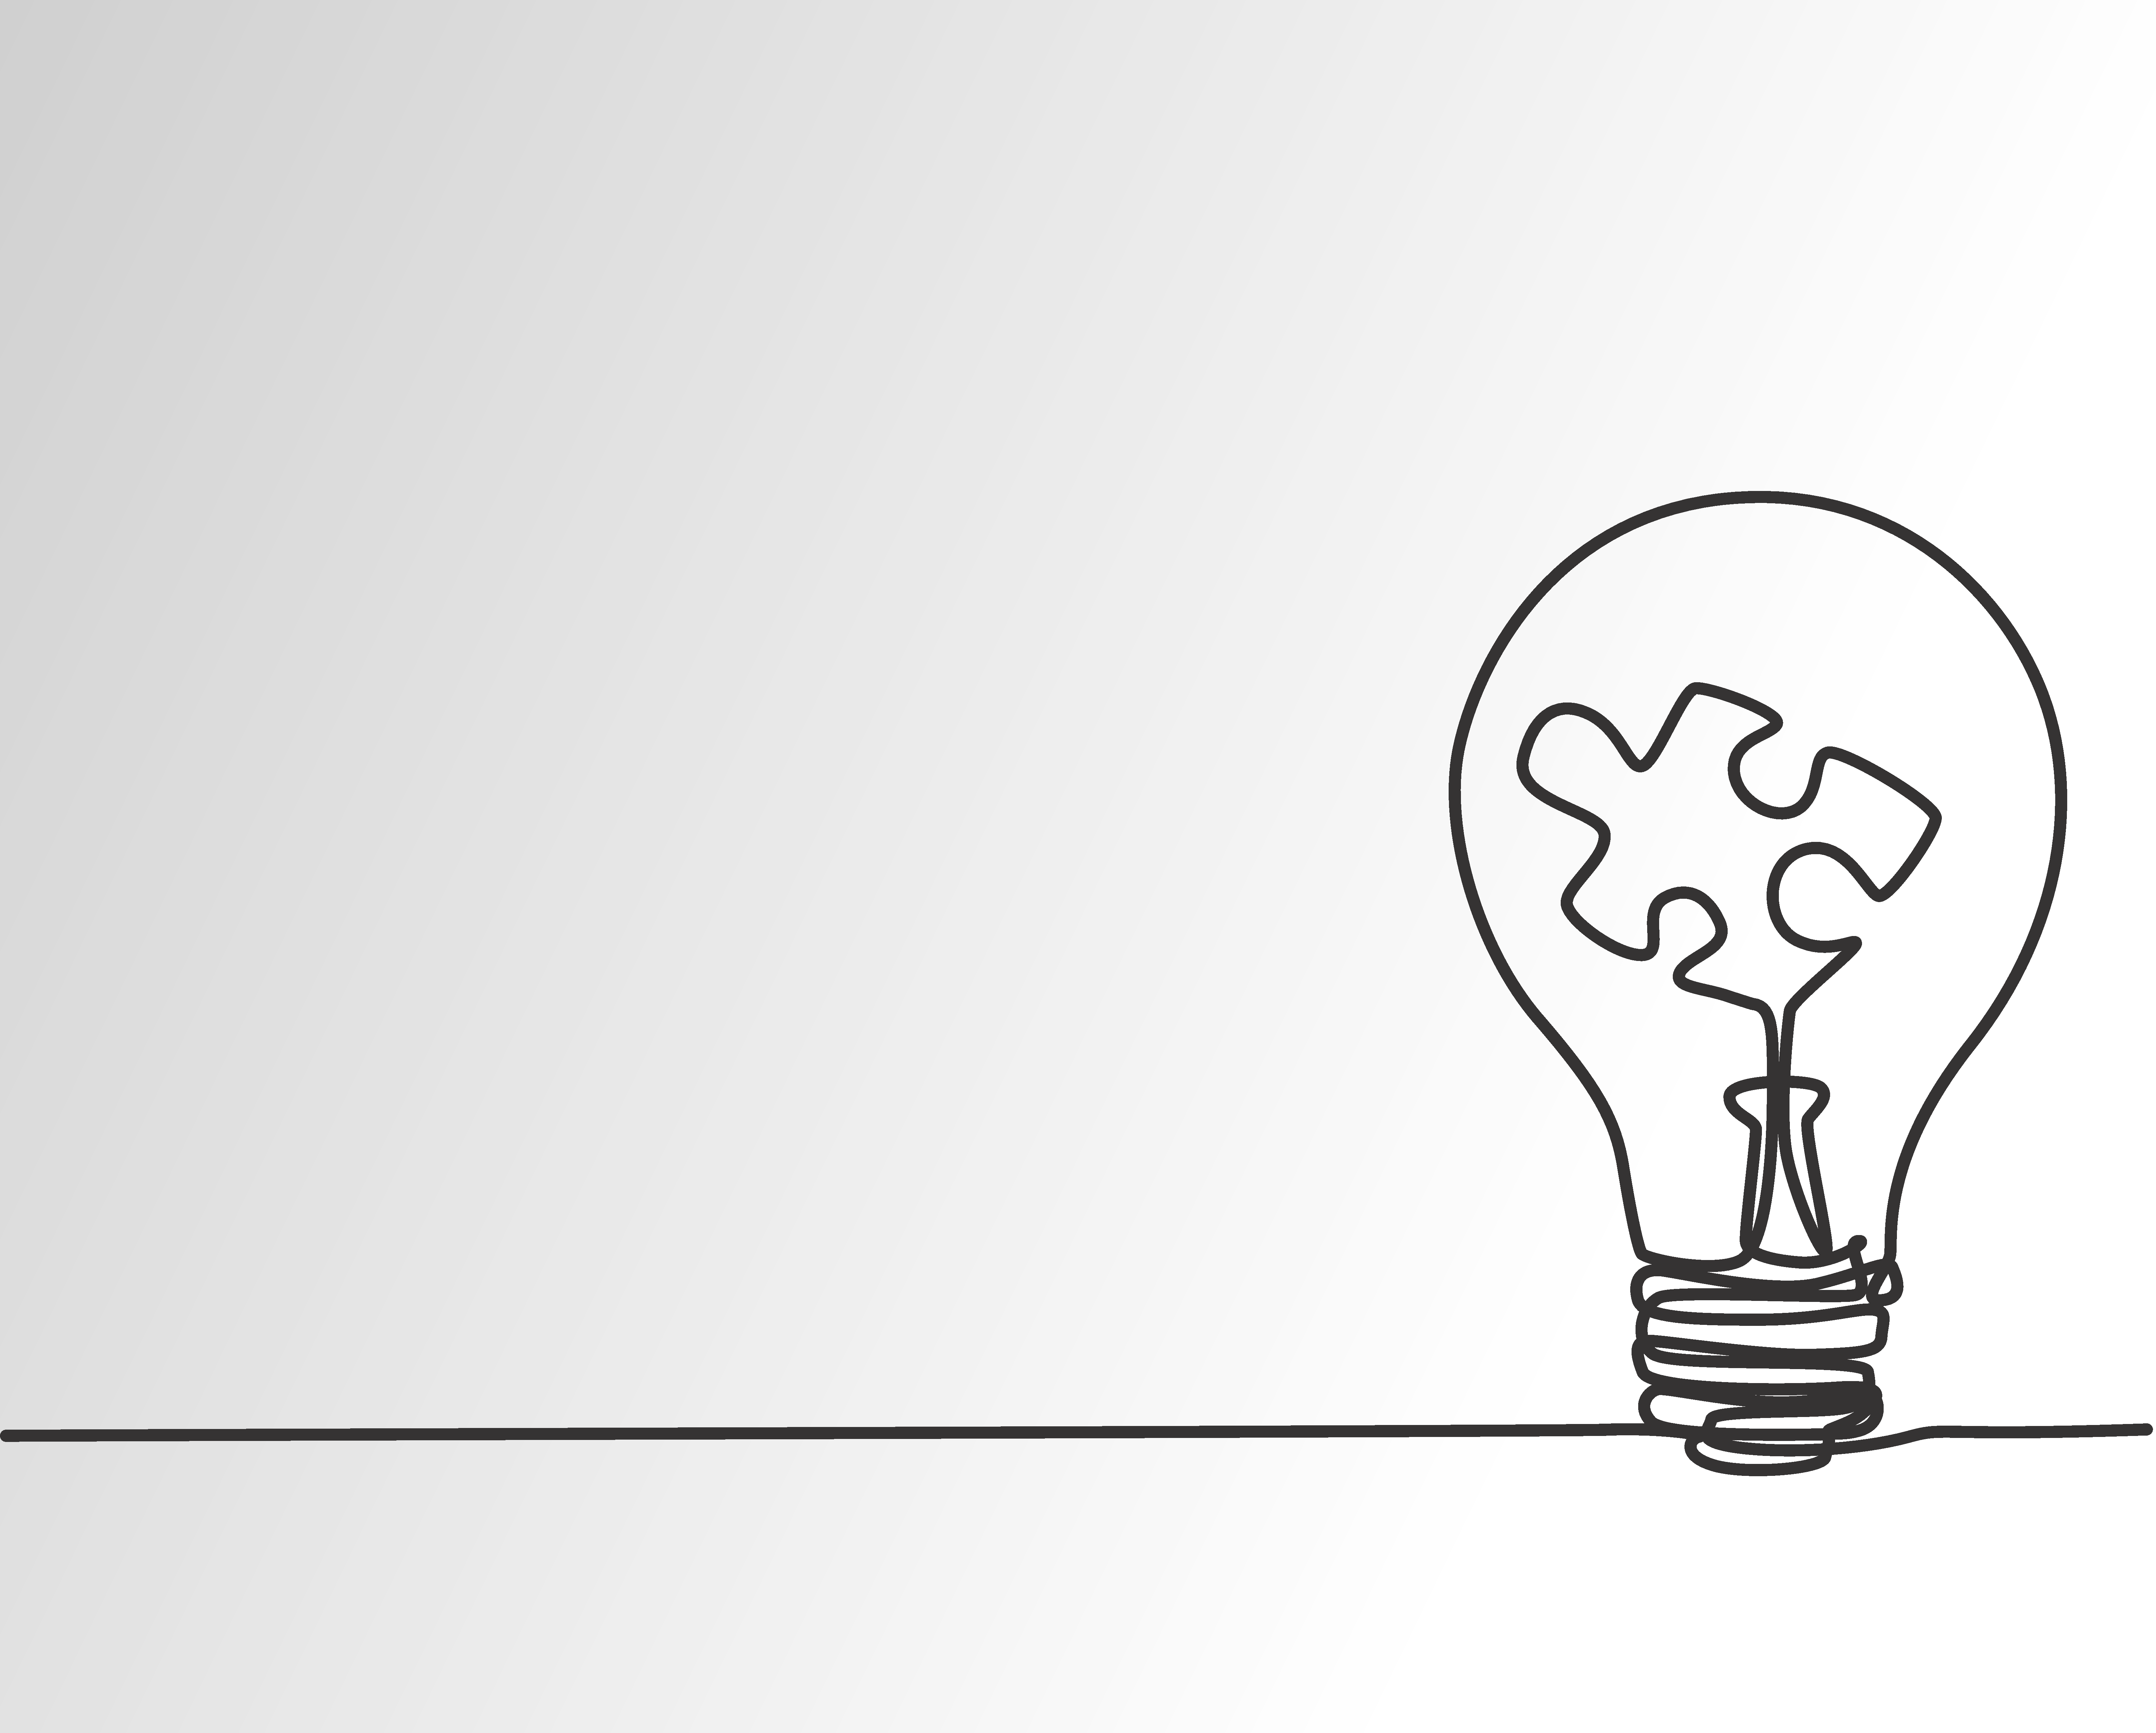
\includegraphics[width=\paperwidth]{figures/main/bulb}}\begin{frame}{Conclusion #1} } { \end{frame} }
% SUMMARY
\newenvironment{summary}[1][] {\begin{frame}{Summary #1} } { \end{frame} }
